\chapter{Acknowledgements}
\label{ch:ack}

Evidence would like to acknowledge as the first thing in this document
the work of Simone Mannori (INRIA, FR), Roberto Bucher (SUPSI Lugano,
CH), Mauro Marinoni, Nicola Serreli, Tullio Facchinetti, and Gianluca
Franchino. These people really made a huge effort to let this
toolchain work on the \flex\ board, spending nights and weekends to
propose you a working system which is fairly easy to use.

This document is just a first step toward a definitive documentation,
so please excuse us for any imprecision or error in this document, and
please report us any problem to let us correct them as soon as possible.

\begin{flushright}
The Evidence Srl Team.
\end{flushright}



%-----------------------------------------------------------------
\chapter{Introduction}
\label{ch:intro}
%-----------------------------------------------------------------

This page contains the information related to the Scilab/Scicos code
generator for the \flex\ board.

The main idea is to {\em develop a single-click digital control
automatic code generation tool for \flex}. 

\begin{figure}[htb]
\begin{center}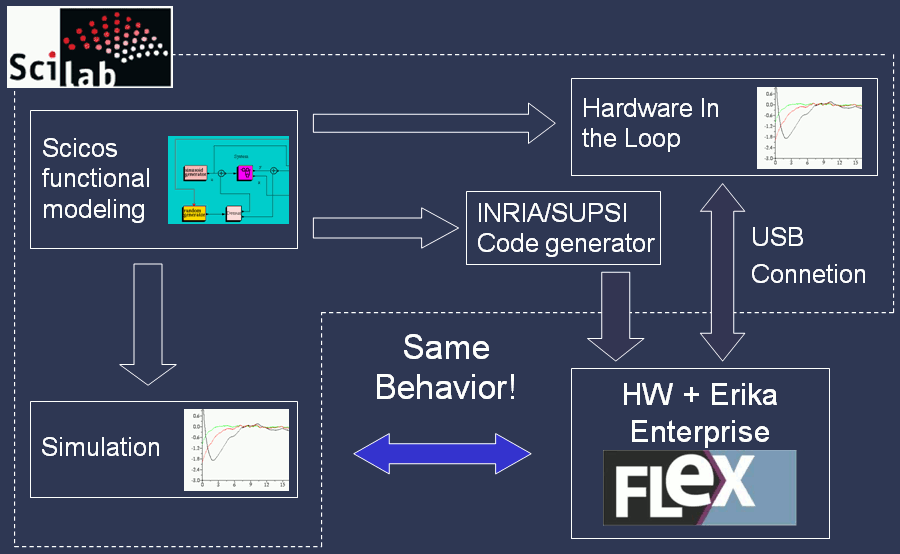
\includegraphics[
  width=10cm, bb=0 0 900 554]{images/scicos_flow.png}\end{center}
\caption{Scilab/Scicos development flow for ERIKA Enterprise and \flex.}
\label{fig:development flow}
\end{figure}


The envisioned design flow, depicted in Figure \ref{fig:development
flow}, is composed by the following steps:
\begin{enumerate}
\item Design of a control system in Scicos;
\item Simulation and tuning of the control system in Scicos;
\item Single-click code generation for ERIKA Enterprise for FLEX;
\item Automatic flashing of the FLEX board;
\item Integration in the Scicos Hardware In the Loop (HIL) support
  using the FLEX USB/wireless connection.
\end{enumerate}

To use The Scilab/Scicos code generator you need at least the
following hardware and software:
\begin{itemize}
\item A \flex\ Board;
\item \ee\ (this document has been written by using \ee\ GPL version 1.4.3);
\item Microchip MPLAB IDE, and the Microchip C30 compiler (available
  from the Microchip web site);
\item A Microchip ICD2 or any device which can be used to program the
  \flex\ board.
  \begin{note}
    The need for a programmer will be removed soon, because the \flex\
    Full version will host a USB programmer on board.
  \end{note}
\end{itemize}

%-----------------------------------------------------------------
\chapter{Notes for Windows XP and Windows Vista users}
\label{ch:vista}
%-----------------------------------------------------------------

If you are using Windows, and especially if you are using Windows
Vista, please look carefully at the following warnings:

\begin{warning}
Do NOT install the Evidence package in a name containing spaces.
\file{c:/Evidence/Evidence} works.
\end{warning}

\begin{warning}
Do NOT install the Scilab package in a name containing spaces.
\file{c:/Evidence/scilab-4.1.2} works.
\end{warning}

\begin{warning}
If using Vista, be aware that directories like 
\file{c:/Programmi}, \file{c:/Users/Documenti} are not REAL directories but are aliases. DO NOT USE THEM. Put your \rtd\ workspace under \file{c:/Users/yourusername/workspace}.
\end{warning}


%-----------------------------------------------------------------
\chapter{Install steps}
\label{ch:install}
%-----------------------------------------------------------------

To install the Scilab/Scicos code generator toolchain, please follow
the steps described in the following paragraphs:

\begin{enumerate}
\item If you have installed a previous version of \ee, please save any
  modification done to the Evidence install directory, which is
  typically stored in the directory
  \const{c:/Evidence/Evidence};
\item If you have installed a previous version of \ee, please
  uninstall it by pressing on the \const{Uninstall} menu item in the
  in the \const{Evidence} menu. Then, please remove by hand everything
  which has been left on your \const{Evidence} directory.
\item Download \ee\ 1.4.3 from the Evidence web site at the following URL:
%%%
%%%  Note: a longer URL, one that could have a longer life cycle
%%%   that the one used here below inside \url{} is: 
%%%   "http://erika.tuxfamily.org/index.php?option=com_content&view=article&id=90&Itemid=74"
%%%
  \url{http://erika.tuxfamily.org/scilabscicos.html}.


\item Install \ee\ 1.4.3 as explained in the documentation available
  on the Evidence web site, and in particular in the Erika Enterprise
  Tutorial for \dspic. Use \file{c:/Evidence/Evidence} as install directory.
\item Please follow exactly the instructions at the previous point. In
  particular, please remind to install the Microchip MPLABIDE and the
  C30 Compiler before installing \ee.
\item Download the \const{scicos_pack_v6.zip} from the Evidence web site.
\item Unzip the file on the desktop. A set of directories are created:
%  \const{Evidence}, 
  \const{scicos_examples}, \const{scilab}, and \const{user}. You need
  to copy these directories in various positions on your hard disk.
%\item Copy the contents of the \const{Evidence} directory inside
%  \const{C:/<programfiles>/Evidence}. This copy will add:
%  \begin{itemize}
%  \item the \const{contrib} directory inside the \const{ee} directory,
%    which includes the Scicos library;
%  \item a working standalone code generator for \ee\ (the one shipped
%    with \ee\ 1.4.0 is broken);
%  \item a template which is used during the code generation process
%    software generated by Scilab/Scicos.
%  \end{itemize}
\item Please check that the file
  \const{c:/Evidence/Evidence/bin/rtd_config.properties}
  contains meaningful settings for your installation. Possible
  settings are explained in the comments in the properties file. In
  particular, you should specify the correct location of the Microchip
  C30 and ASM30 tools. The following is an example for an italian
  installation:
  \begin{lstlisting}
preference_pic30__path_for_asm_compiler = <same line>
  C:\\Programmi\\Microchip\\MPLAB ASM30 Suite
preference_pic30__path_for_gcc_compiler = <same line>
  C:\\Programmi\\Microchip\\MPLAB C30
  \end{lstlisting}

  Please note to use a double backslash and not a
  single backslash!
\begin{warning}
If you are using Windows Vista, put the REAL directory here. For example, in Italian Vista installations \file{c:/Programmi} is an alias to \file{c:/Program Files}. Please use \file{c:/Program Files} and not \file{c:/Programmi}.
\end{warning}

\item Download and install Scilab 4.1.2 binary version for Windows from
  the web site \url{http://www.scilab.org}. Please use an install
  directory {\bf which does not contain spaces}:
  \const{C:/Evidence/scilab-4.1.2} is ok.
\item Erase the \const{contrib} directory inside your Scilab
  installation, and replace it with the \const{scilab/contrib}
  directory you just unzipped. This step copies the code generator and
  the palettes for \flex\ inside the Scicos install directory.
\item Copy the content of the \const{user} directory inside your
  \const{c:/Documents and Settings/username} directory. 
  \begin{warning}
  For Windows Vista users: read \file{c:/Users/username}
  \end{warning}
  This step will
  add a \const{.scilab} file inside the Scilab environment
  directory. The new \const{.scilab} is used to display the palettes
  of the code generator for \flex.

\item Copy the \const{scicos_examples} directory in a useful place,
  e.g. \const {c:/ }.
\item Your Scilab/Scicos installation is now ready to produce code.
\end{enumerate}

%-----------------------------------------------------------------
\chapter{Your first Scicos application}
\label{ch:firstexample}
%-----------------------------------------------------------------

This Chapter will guide you to the creation, compilation and execution
of a first simple Scicos example on a \flex\ board. The example
created in this tutorial can be found in the directory
\const{scicos_examples/led_sin}.

If you are looking for a prebuilt example, go directly to Section
\ref{sec:codegen}.

\section{Creating the Scicos example files}

\begin{enumerate}
\item
  Please start Scicos 4.1.2 from the \const{Start} menu. The Scilab
  window appears.

\item
  Type ``\const{scicos();}'', as showed in Figure
  \ref{fig:scilab_splash}, and press Enter.
%
\begin{figure}[htb]
\begin{center}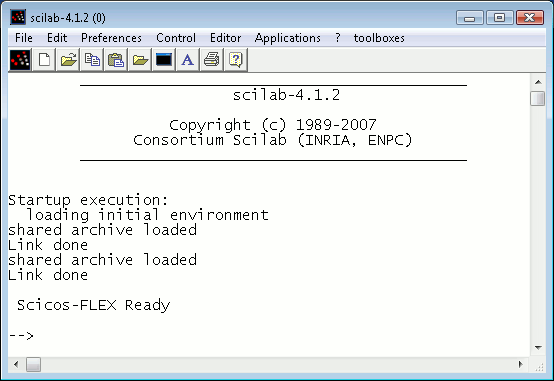
\includegraphics[
  width=10cm, bb=0 0 554 381]{images/scilab_splash.png}\end{center}
\caption{The Scilab splash screen. Type \const{scicos();} to start Scicos.}
\label{fig:scilab_splash}
\end{figure}

\item
  The Scicos windows appears, as showed in Figure
  \ref{fig:scicos_splash}.
%
\begin{figure}[htb]
\begin{center}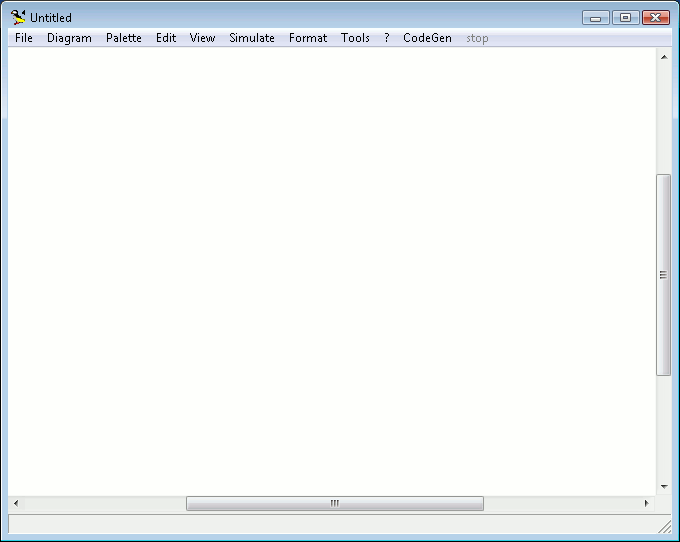
\includegraphics[
  width=10cm, bb=0 0 680 542]{images/scicos_splash.png}\end{center}
\caption{The Scicos splash screen.}
\label{fig:scicos_splash}
\end{figure}

\item
  Select \const{Palettes} from the \const{Edit} menu, as showed in Figure
  \ref{fig:palette_menu}.
%
\begin{figure}[htb]
\begin{center}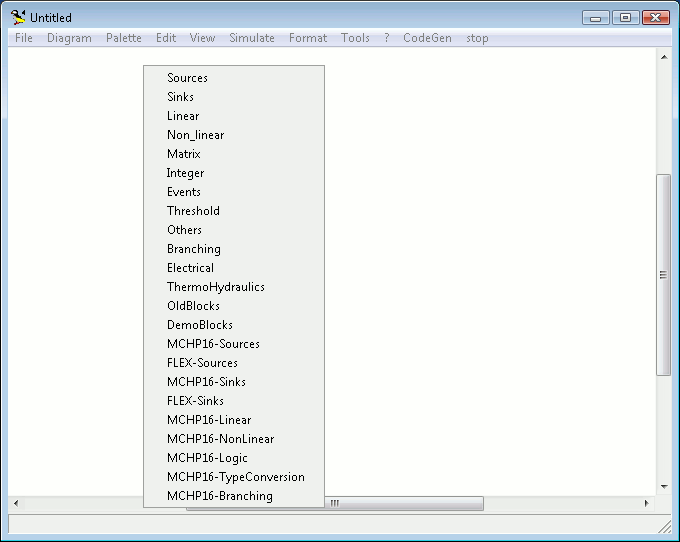
\includegraphics[
  width=10cm, bb=0 0 680 542]{images/palette_menu.png}\end{center}
\caption{The \const{Edit} menu. Select \const{Palettes}}
\label{fig:palette_menu}
\end{figure}

\item
  A little list appear in place of the menu. Select \const{FLEX-Sinks},
  as showed in Figure
  \ref{fig:palette_menu2}.
%
\begin{figure}[htb]
\begin{center}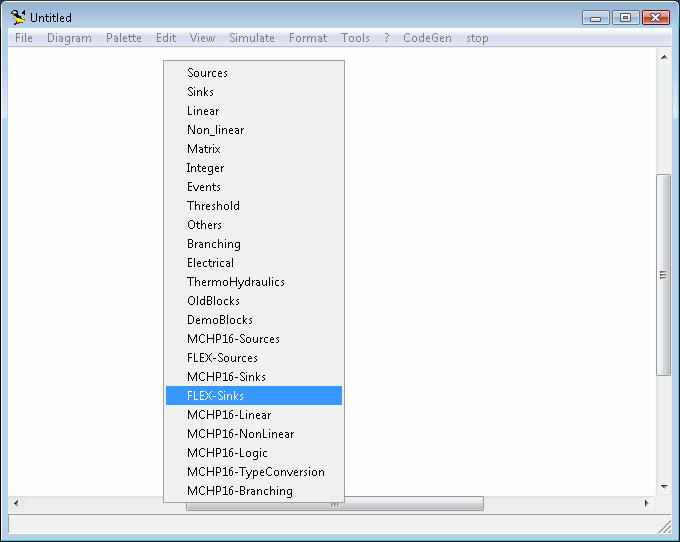
\includegraphics[
  width=10cm, bb=0 0 680 542]{images/palette_menu2.png}\end{center}
\caption{The Palette list.}
\label{fig:palette_menu2}
\end{figure}


\item
  A windows appears, with some sink blocks specific for the
  \flex\ board (see Figure \ref{fig:palette}) (a complete list of the available blocks is available at the end of this document).
%
\begin{figure}[htb]
\begin{center}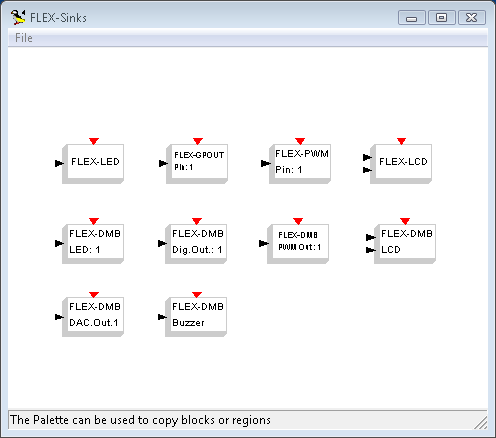
\includegraphics[
  width=10cm, bb=0 0 496 438]{images/palette.png}\end{center}
\caption{The dsPIC Palette.}
\label{fig:palette}
\end{figure}

\item
  Single click on the \const{FLEX-LED} block. The window selection moves to
  the Scicos window. The mouse now becomes a white rectangle of the
  dimension of the \const{LED} block. Single click somewhere in the
  white part of the window. A \const{LED} block is dropped in the
  diagram, like in Figure \ref{fig:led}.
%
\begin{figure}[htb]
\begin{center}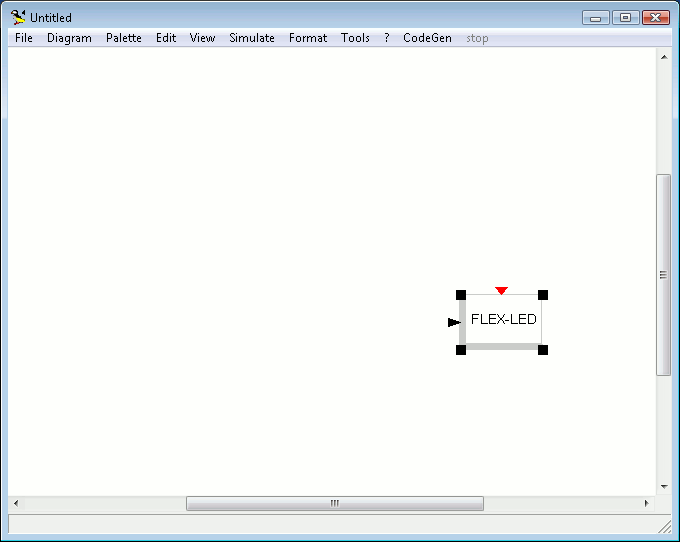
\includegraphics[
  width=10cm, bb=0 0 680 542]{images/led.png}\end{center}
\caption{The \const{LED} block is dropped in the design window.}
\label{fig:led}
\end{figure}

\begin{note}
If you need to move a block, go over it with the mouse, press
\const{m}, then move the block and click on the new position!
\end{note}

\begin{note}
If you need to delete a block or a line, go over it with the mouse,
then press \const{d}!
\end{note}

\begin{note}
If some garbage appears on the diagram windos, don't panic! Just press
\const{r}!
\end{note}

\item
  Open the MCHP16-Sources palette, and repeat the same with the \const{Sine} block, placing it on the left
  of the \const{LED} block, as in Figure \ref{fig:sineled}.
%
\begin{figure}[htb]
\begin{center}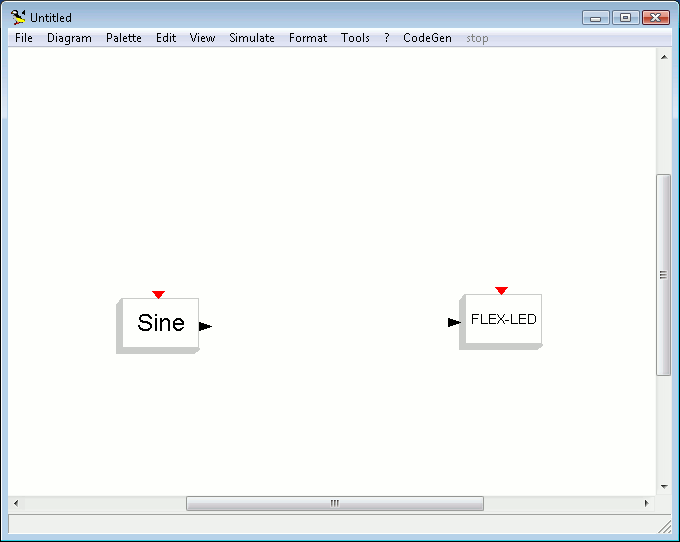
\includegraphics[
  width=10cm, bb=0 0 680 542]{images/sineled.png}\end{center}
\caption{Place the \const{Sine} block to the left of the \const{LED} block.}
\label{fig:sineled}
\end{figure}

\item
  Link the black triangle of the \const{Sine} block to the black
  triangle of the \const{LED} block. To do that, press \const{l}, then
  single click on the triangle of the \const{Sine} block (the {\em
  source}), then click again on the triangle of the \const{LED} block
  (the {\em sink}). See Figure \ref{fig:link}.
%
\begin{figure}[htb]
\begin{center}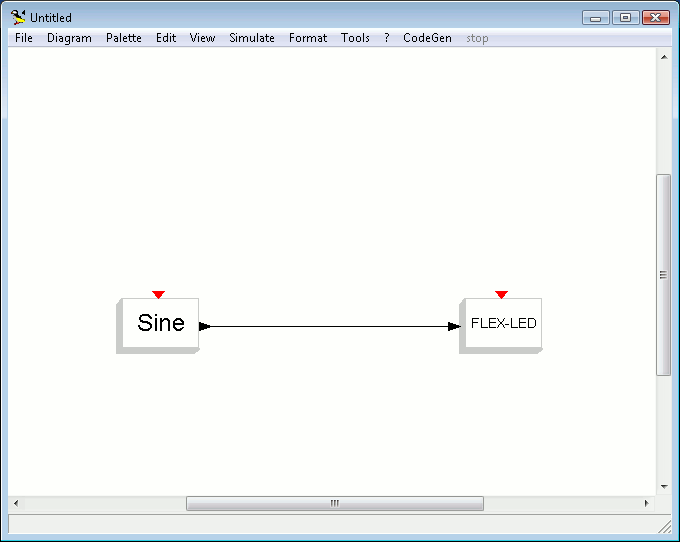
\includegraphics[
  width=10cm, bb=0 0 680 542]{images/link.png}\end{center}
\caption{\const{Sine} and \const{LED} are now linked.}
\label{fig:link}
\end{figure}

\item
  From the \const{MCHP16-Sources} Palette, which can be found il the
  palette list (see Figure \ref{fig:palette_menu2}. Choose the red
  clock, and put it on the diagram as shown in Figure \ref{fig:clock}.
%
\begin{figure}[htb]
\begin{center}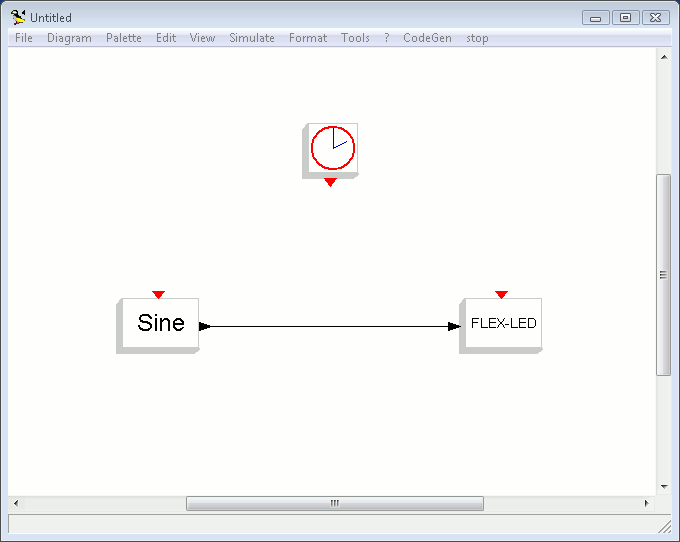
\includegraphics[
  width=10cm, bb=0 0 680 542]{images/clock.png}\end{center}
\caption{Put the \const{Clock} block over the \const{Sine} and \const{LED} blocks.}
\label{fig:clock}
\end{figure}

\item
  Now connect the clock signal to the two blocks. To do that, single
  click on the red triangle of the \const{clock} block, then single
  click below it, then single click over the \const{Sine} block, then
  click on the red triangle of the \const{Sine} block. After that,
  single click on the line below the \const{clock} block, then over
  the \const{LED} block, then on the red triangle of the \const{LED}
  block. The result is shown in Figure \ref{fig:redlink}

%
\begin{figure}[htb]
\begin{center}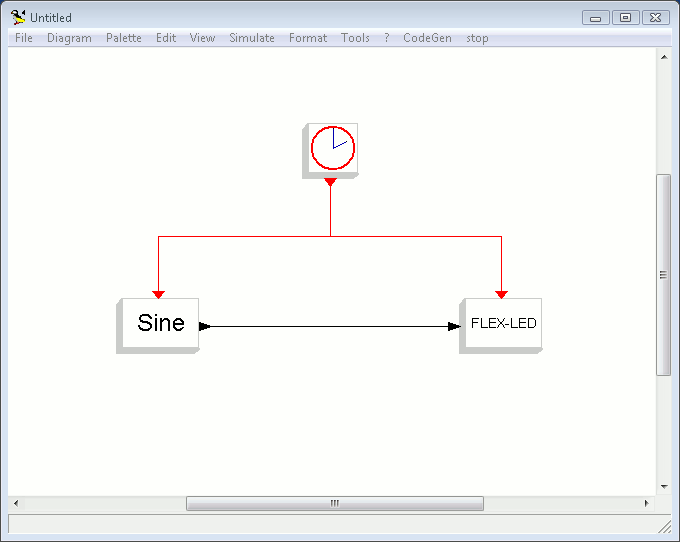
\includegraphics[
  width=10cm, bb=0 0 680 542]{images/redlink.png}\end{center}
\caption{The \const{Clock} block is connected to the \const{Sine} and
\const{LED} blocks.}
\label{fig:redlink}
\end{figure}

\item
  Single click on the \const{Clock} block. Its properties window
  appears. Leave them untouched, and press \const{OK}. You can do the
  same on the \const{Sine} block. Figure \ref{fig:clockproperties} and
  \ref{fig:sineproperties} show these windows.
%
\begin{figure}[htb]
\begin{center}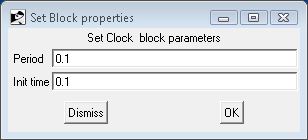
\includegraphics[
  width=6cm, bb=0 0 308 140]{images/clockproperties.png}\end{center}
\caption{The \const{Clock} block properties.}
\label{fig:clockproperties}
\end{figure}
%
\begin{figure}[htb]
\begin{center}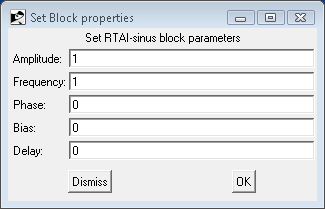
\includegraphics[
  width=6cm, bb=0 0 325 209]{images/sineproperties.png}\end{center}
\caption{The \const{Sine} block properties.}
\label{fig:sineproperties}
\end{figure}

\item
  The code generator can produce code which only comes from a special
  block named {\em Super Block}. For this reason, we need to create a
  Super Block enclosing the \const{Sine} and the \const{LED}
  blocks. To do that, select the \const{Region to Super Block} menu
  item from the \const{Diagram} menu (see Figure
  \ref{fig:region2sb}). Then, draw a selection which includes the
  \const{Sine}, the \const{LED}, and the red lines in a way that only
  {\em one} red line exits the selection, as shown in Figure
  \ref{fig:sb}.
%
\begin{figure}[htb]
\begin{center}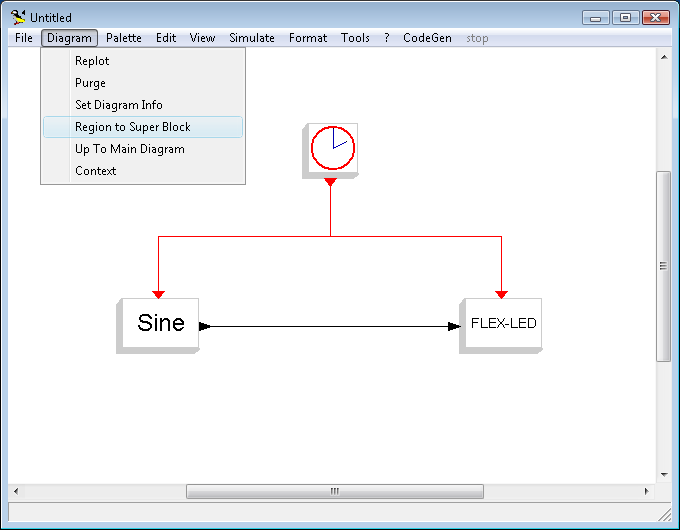
\includegraphics[
  width=10cm, bb=0 0 680 530]{images/region2sb.png}\end{center}
\caption{The Region to Super Block menu item.}
\label{fig:region2sb}
\end{figure}
%
\begin{figure}[htb]
\begin{center}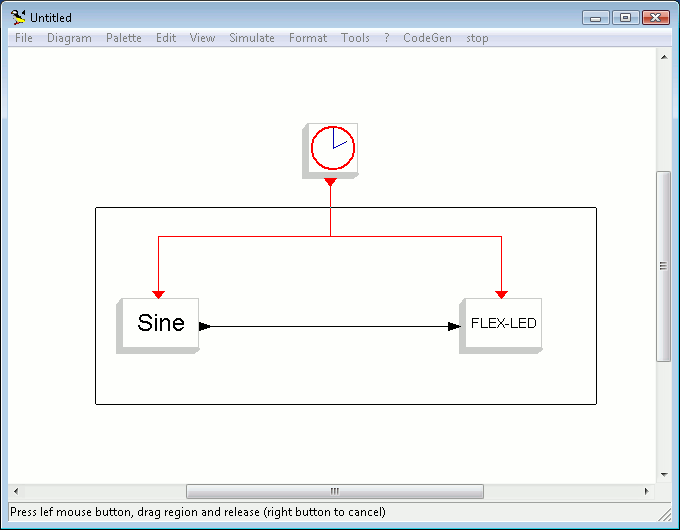
\includegraphics[
  width=10cm, bb=0 0 680 530]{images/sb.png}\end{center}
\caption{The selection made to create a Super Block.}
\label{fig:sb}
\end{figure}

\item
  As a result, a Super Block is created (see Figure \ref{fig:sb1}),
  which contains the \const{Sine} and \const{LED} blocks. To see these
  blocks, just single click on the Super Block, and another window
  will appear (see Figure \ref{fig:sb2}). Please note that this window
  is very similar to the previous one except that the \const{clock}
  object is substituted by a placeholder signed with the number 1.
%
\begin{figure}[htb]
\begin{center}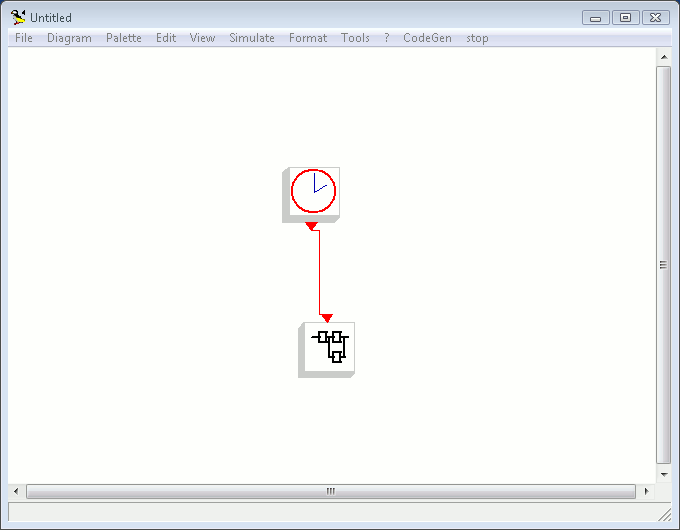
\includegraphics[
  width=10cm, bb=0 0 680 530]{images/sb1.png}\end{center}
\caption{The Super Block.}
\label{fig:sb1}
\end{figure}
%
\begin{figure}[htb]
\begin{center}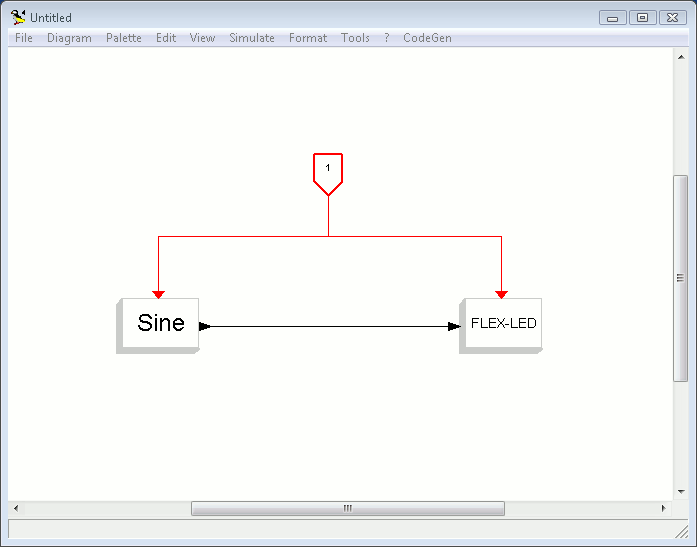
\includegraphics[
  width=10cm, bb=0 0 697 547]{images/sb2.png}\end{center}
\caption{The contents of the Super Block.}
\label{fig:sb2}
\end{figure}

\begin{note}
The Diagram containing the Super Block is disabled when the Super
Block diagram is displayed. Only one window can be enabled at a time
in Scicos. The limitation will be removed in the next version of
Scicos.
\end{note}

\item
  It is now time to save the two diagrams. From the \const{File}
  menu, choose \const{Save as}. Save the
  diagram containing the Super Block as \const{led_sin.cos}.

\end{enumerate}

\section{Generating dsPIC code from a Scicos Diagram}
\label{sec:codegen}

It is now time to generate the code for the example we just created.

\begin{note}
  A copy of the file created in the previous steps is included inside the
  \const{scicos_examples/led_sin} directory. To open it, double click
  on the \const{scicos_examples/led_sin/led_sin.cos} file.
\end{note}

\begin{enumerate}
\item
  Select \const{EmbCodeGen} from the \const{CodeGen} menu (see Figure
  \ref{fig:codegen1}).
%
\begin{figure}[htb]
\begin{center}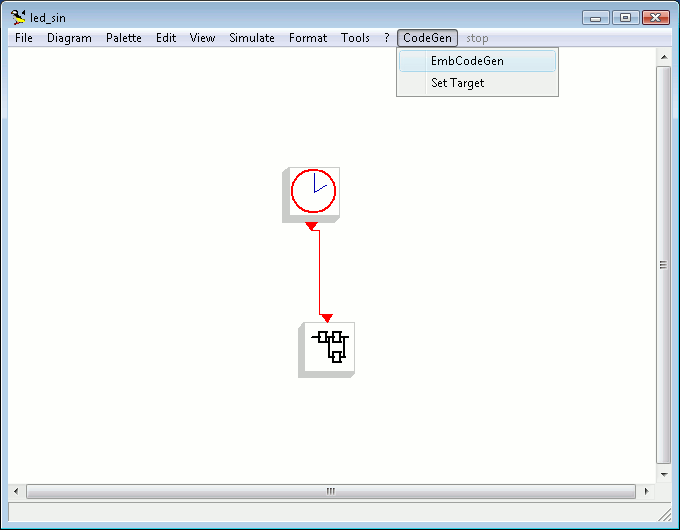
\includegraphics[
  width=10cm, bb=0 0 680 530]{images/codegen1.png}\end{center}
\caption{The \const{CodeGen} menu.}
\label{fig:codegen1}
\end{figure}

\item
  A window appear, like the one in Figure \ref{fig:codegen2}. You can
  specify the directory where all the files will be created by
  modifying the \const{Created files Path} textbox. Please leave the
  other options unchanged.
%
\begin{figure}[htb]
\begin{center}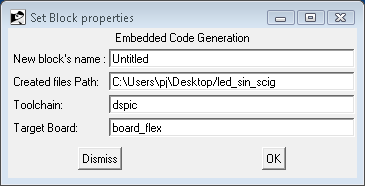
\includegraphics[
  width=6cm, bb=0 0 365 186]{images/codegen2.png}\end{center}
\caption{The \const{EmbCodeGen} dialog box.}
\label{fig:codegen2}
\end{figure}

\item
  Press \const{Ok}. As a result, a set of files are generated in the
  output directory.

\item
  Then, Scicos automatically opens a console window, running in it the
  following commands:
  \begin{itemize}
  \item the \rtd\ template generator to instantiate the Scicos
    template application;
  \item the \rtd\ standalone code generator to produce the \ee\
    configuration files from the generated OIL file;
  \item the \const{make} application to compile the code.
  \end{itemize}

\item
  The result of the code generation process is depicted in Figure
  \ref{fig:console}. The executable file is named \const{pic30.elf}
  and it is located inside the \file{Debug} directory as usual for all
  the \ee\ applications.
%
\begin{figure}[htb]
\begin{center}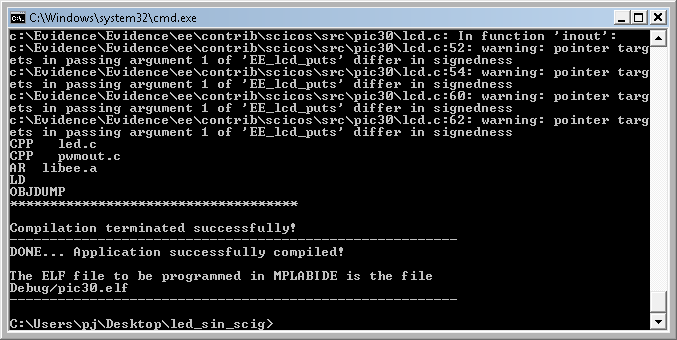
\includegraphics[
  width=10cm, bb=0 0 677 340]{images/console.png}\end{center}
\caption{The compilation console.}
\label{fig:console}
\end{figure}

\begin{warning}
If the error depicted in Figure \ref{fig:license_problem} appears, it
is likely that you have an expired license of the Microchip C30
compiler Student Edition.

Try putting to \const{true} the following two lines inside the
\const{c:/<programfiles>/Evidence/bin/rtd_config.properties} file, to
select the Evidence compiler recompiled from the sources.

\begin{lstlisting}
preference_pic30__use_evidence_compiler_4_deps = true
preference_pic30__use_evidence_compiler_4_compile = true
\end{lstlisting}
\end{warning}
%
\begin{figure}[htb]
\begin{center}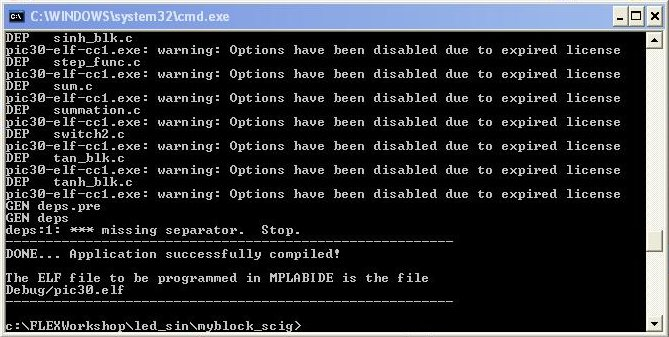
\includegraphics[
  width=10cm, bb=0 0 669 337]{images/license_problem.jpg}\end{center}
\caption{License problem when compiling.}
\label{fig:license_problem}
\end{figure}

\item
  You can now program your application on your \flex\ board. To do
  that, you need to open MPLABIDE as you usually do to program other
  \ee\ applications. Please refer to the \ee\ tutorial for \dspic\
  for more information.
  
  \begin{warning}
    If the ELF file fails to import on the MPLABIDE, try to use the
    C30 compiler recompiled from the Microchip sources by setting the
    following variables in the file
    \const{c:/<programfiles>/Evidence/bin/rtd_config.properties}:
    \begin{lstlisting}
preference_pic30__use_evidence_compiler_4_deps = true
preference_pic30__use_evidence_compiler_4_compile = true
    \end{lstlisting}
  \end{warning}

\item
  Running the code on your \flex\ board has the following behavior: the
  system led on the board flashes with a period of 20 seconds, and a
  duty cycle of around 6 seconds over 20. The explanation is the
  following: 
  \begin{itemize}
  \item
    The system works like a synchronous control system, with a
    sampling frequency of $0.1 s$ (see Figure
    \ref{fig:clockproperties}).
  \item
    The \const{Sine} block output is a sinus with a frequency of
    $0.05$, which correspond to a period of $20 s$ (see Figure
    \ref{fig:sineproperties}).
  \item
    The \const{LED} block is directly linked to the system led, and is
    programmed to put on the system led when its input is greater than
    $0.5$.
  \item
    Looking at Figure \ref{fig:graphic}, it is clear that the sinus
    has a value greater than $0.5$ for around a third of its
    period. Given that, the system led is on for around 6 seconds over
    20.
  \end{itemize}
%
\begin{figure}[htb]
\begin{center}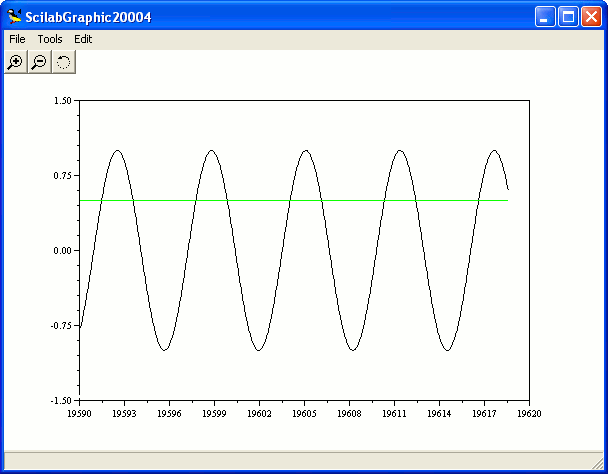
\includegraphics[
  width=10cm, bb=0 0 608 474]{images/graphic.png}\end{center}
\caption{A graphic of a Sine and of a constant value $0.5$.}
\label{fig:graphic}
\end{figure}

\end{enumerate}
  
%-----------------------------------------------------------------
\chapter{Internals of the genaretd code}
\label{ch:internals}
%-----------------------------------------------------------------

\section{Templates and customization of the generated application}

The default application wich is generated by the Scicos embedded code
generator for \dspic\ generates a basic application which uses \ee\
with the FP kernel, a periodic task and an Alarm triggered by a timer
interrupt to activate it.

In general, it is likely that advanced users would like to customize
the application which is generated by the code generator, to add other
activities to be executed concurrently with the code generated from
the Scicos design. Examples of this activities could be for example
background activities for reporting, supervision, display, debug, and
so on.

Implementing such variations is very easy, because the application
scheleton used by the code generator is contained inside a \rtd\
template. In particular, the default template is the
\const{pic30_empty_scicos} template stored inside the
\file{examples/pic30/pic30_scicos} directory under the \ee\ install
tree. The user can add a new template using the following
steps:
\begin{enumerate}
\item Copy the \file{examples/pic30/pic30_scicos} directory in another
  location under the \file{examples} directory;

\item Change the \const{ID} of the template by modifying the
  \file{template.xml} file contained inside the directory. The
  \const{ID} is specified in the second line of the XML file as
  follows:

\begin{lstlisting}
<evidence_example version="1" ID="pic30_empty_scicos">
\end{lstlisting}

\item Change the files included in the new template. If you need to
  add a new file, please remember to add it in the corresponding list
  in the \file{template.xml} file.
\end{enumerate}

Finally, specify the new template when generating the code in the
\const{Template} textbox in Figure \ref{fig:codegen2}.

\section{Assumptions of the default template}
The code generated by the Scilab/Scicos code generator for \flex\ uses
the template named \const{pic30_empty_scicos}, and has the following
symplifing assumptions:

\begin{enumerate}
\item There is a single sampling time $T_s$ in the system;
\item $T_s$ is forced to 1 ms;
\item Every sampling time specified by the user under the Scicos
  design will be rounded to a multiple of a millisecond;
\item An \ee\ counter is linked to the a periodic timer;
\item The periodic timer used in the dsPIC hardware is set to raise an
  interrupt every 1 ms;
\item An \ee\ alarm is attached to the counter, to periodically
  activate a task;
\item The task body just calls the routines generated by the Scicos
  code generator. Which executes the functions you specified in the
  design;
\item The PWM object has a fixed period of 1 ms. This means that if
  the sampling period is a multiple of $T_s$, then the PWM will repeat
  the same duty cycle until the PWN value is changed;
\item The A/D converter always works ``on demand'', meaning it always
  executes the following steps:
  \begin{itemize}
    \item selects a channel;
    \item starts the conversion;
    \item waits for the end of the conversion (typically max $10 \mu sec$)
    \item it converts the result in a value from $0.0 V$ and $3.3 V$
  \end{itemize}
\item To speedup the compilation process, the default configuration does not produce the dependency files and the \file{.src} file from every \file{.c} file.
\end{enumerate}
